\chapter{Performance Evaluation} % Main chapter title
\label{chapter6_pe}
In this chapter we describe the environment and the test scenarios we implemented in order to record the performance of our system. In table ~\ref{server_ch} we present the characteristics of our framework witch we use in our tests. \par 
	The capacity of the server's RAM is 8 GB. The operating system we selected for our tests is Debian 8 (Jessie) release. We used two different tools for the benchmarking of our system's performance. The first tool is the ab Apachee HTTP server benchmarking tool, that enables us to send multiple requests  per second with fixed number of total requests. The second tool we used is the wrk, which allows us to send concurrent requests for a specific amount of time with timeout adjustment. With the aid of these tools we implemented two test scenarios, the results of which are presented below. \par 


\begin{table}[]
\centering
\begin{tabular}{|c|c|}
\hline
\rowcolor[HTML]{34FF34} 
\textbf{Architecture}        & x86\_64                              \\ \hline
\rowcolor[HTML]{FFFFFF} 
\textbf{CPU op-mode(s)}      & 32-bit, 64-bit                       \\ \hline
\rowcolor[HTML]{34FF34} 
\textbf{Byte Order}          & Little Endian                        \\ \hline
\rowcolor[HTML]{FFFFFF} 
\textbf{CPU(s)}              & 8                                    \\ \hline
\rowcolor[HTML]{34FF34} 
\textbf{On-line CPU(s) list} & 0-7                                  \\ \hline
\rowcolor[HTML]{FFFFFF} 
\textbf{Thread(s) per core}  & 1                                    \\ \hline
\rowcolor[HTML]{34FF34} 
\textbf{Core(s) per socket}  & 4                                    \\ \hline
\rowcolor[HTML]{FFFFFF} 
\textbf{Model}               & 23                                   \\ \hline
\rowcolor[HTML]{34FF34} 
\textbf{Model name}          & Intel(R) Xeon(R) CPU,X5450,@ 3.00GHz \\ \hline
\end{tabular}
\caption{Server characteristics}
\label{server_ch}
\end{table}


\section{First Test}
In the first test we selected some indicative server routes for measurement. In order to measure their performance, we select a predefined number of requests to be sent to the server, changing the number of concurrent requests in each iteration. The criterion of the server's performance is the total time for the response of all the requests. The smaller the time, the better. The results are presented in figure~\ref{experiment_fig}. \par 
 
\begin{figure}
\centering
\begin{subfigure}{1\textwidth}
  \centering
  \centerline{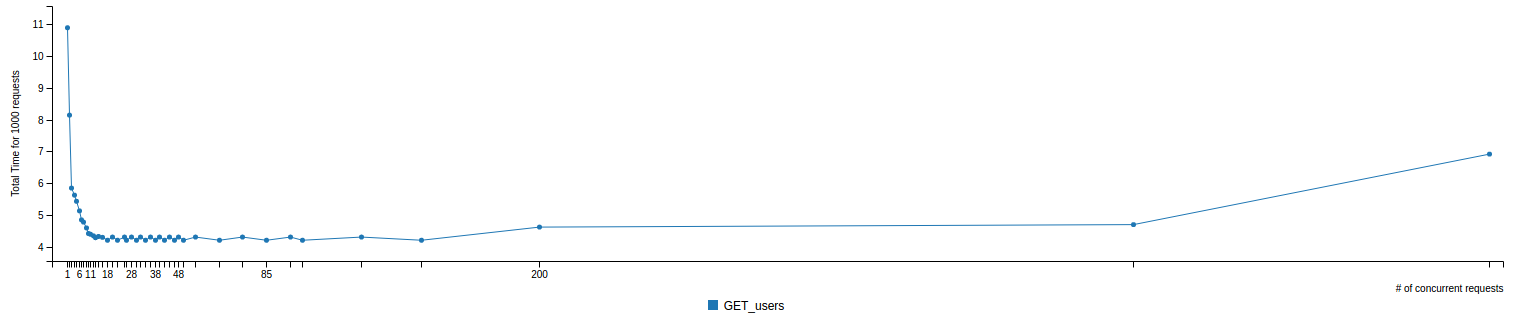
\includegraphics[width=1.2\linewidth]{get_users.png}}
  \caption{GET users route experiment}
\end{subfigure}
\begin{subfigure}{1\textwidth}
  \centering
  \centerline{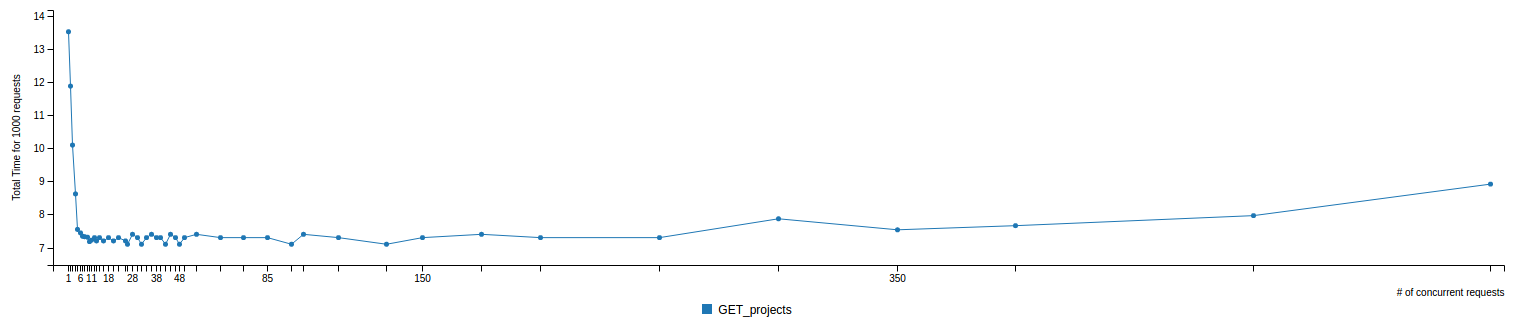
\includegraphics[width=1.2\linewidth]{post_projects.png}}
  \caption{POST projects route experiment}
\end{subfigure}
\begin{subfigure}{1\textwidth}
  \centering
  \centerline{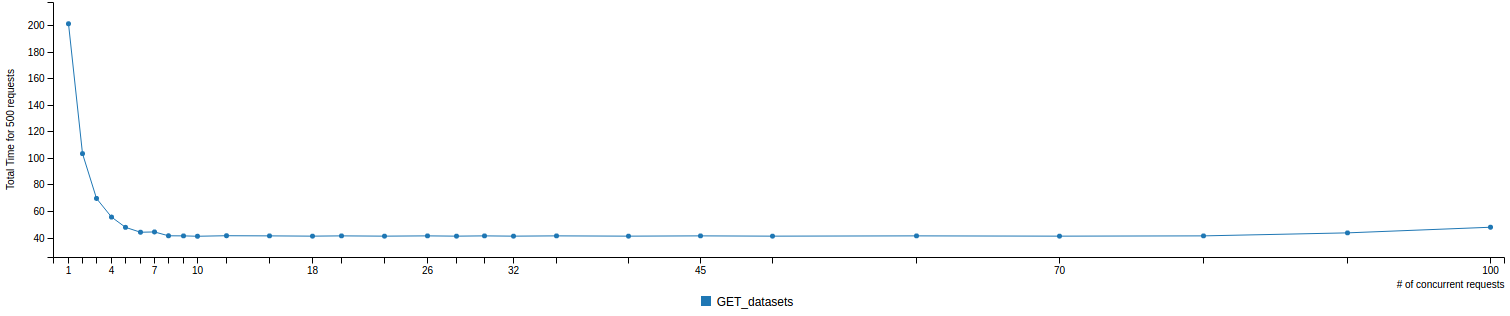
\includegraphics[width=1.2\linewidth]{get_datasets.png}}
  \caption{GET datasets route experiment}
\end{subfigure}
\begin{subfigure}{1\textwidth}
  \centering
  \centerline{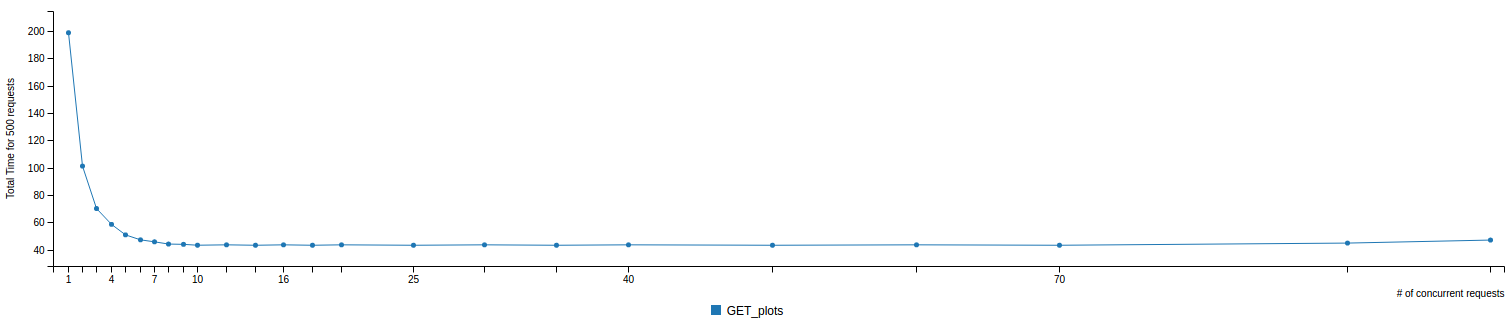
\includegraphics[width=1.2\linewidth]{get_plots.png}}
  \caption{GET plots route experiment}
\end{subfigure}
\caption{Total time for all requests / number of concurrent requests figure}
\label{experiment_fig}
\end{figure}


As we notice all the subfigures follow a specific pattern. Initially in all the subfigures the total time for the response of all the requests is considerably higher, compared to the following values of the diagrams. This is due to the low initial concurrency, which causes a delay until the requests are sent. That is, the client cannot send a big concurrent load. In the case that "c=1", each request is sent after the completion of the previous sending, which explains the relatively high initial values. \par 
	Following, we observe in all the diagrams a stabilization of the total time of serving the requests, as the "c" increases. This is partially due to the adequate load the client provides, so that there is no delay of the sending of the requests, but also because the server has enough time to respond without any delay. \par 
	At the end of the subfigures we notice that the total time for serving the requests starts to increase gradually. The reason is that the number of concurrent requests sent by the client is now too high to be served by the server, and this is the cause of the delay. \par 
	We observe significant differences between the values of the diagrams, the most important being in the routes where python is used. To execute these routes, new child processes must be spawned. As the number of the concurrent requests increases, the spawned child processes block the function of the server. This is how the higher time values in serving the requests are explained.  

	
\section{Second Test}
The basic characteristic of the second test scenario is the timeout value. A timeout occurs when the server fails to serve a request in a specific time period from the moment it was sent. In this test we set a relatively small timeout limit of two seconds and define each iteration in ten seconds per concurrency value. Gradually we raise the concurrency value and we calculate the number of served requests per second. The test scenario is finished when the first timeout error occurs. The results are presented in figure ~\ref{experiment_fig2}. \par 


\begin{figure}
\centering
\begin{subfigure}{1\textwidth}
  \centering
  \centerline{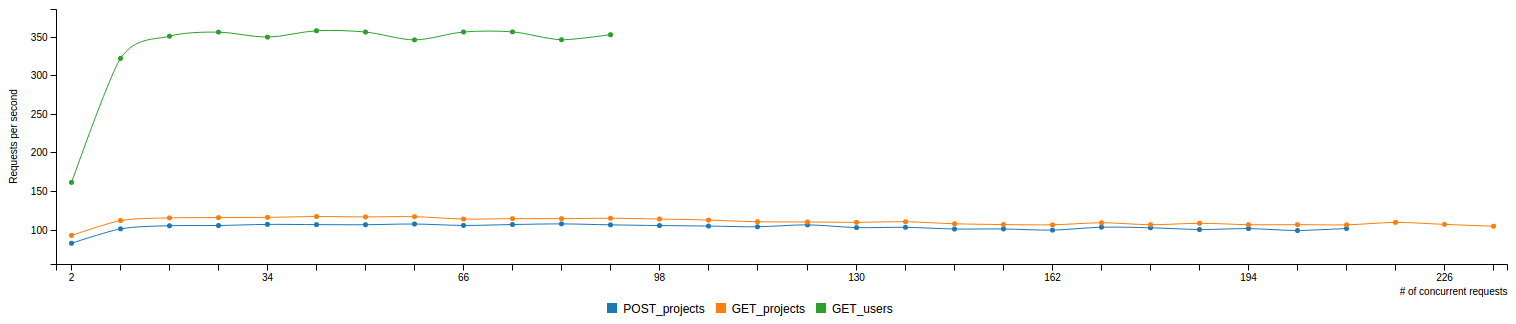
\includegraphics[width=1.2\linewidth]{error1.png}}
  \caption{Second experiment result}
\end{subfigure}
\begin{subfigure}{1\textwidth}
  \centering
  \centerline{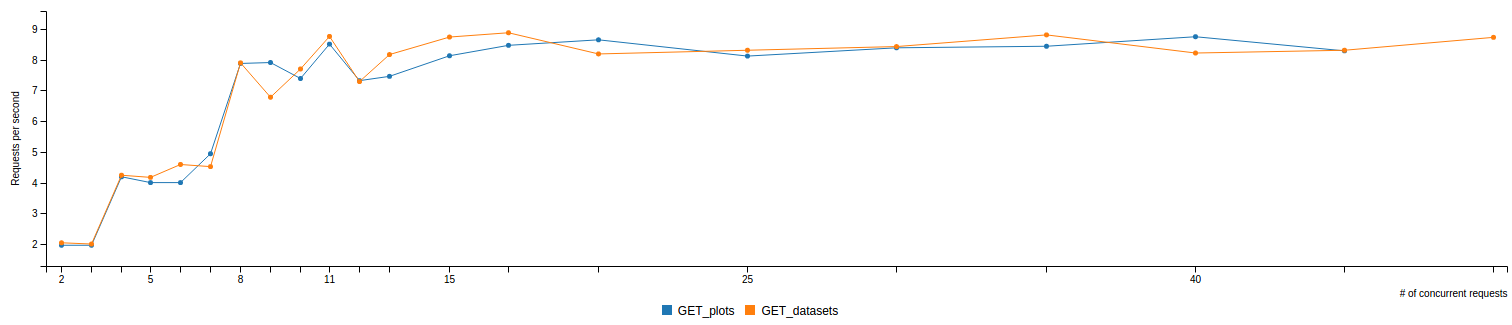
\includegraphics[width=1.2\linewidth]{error2.png}}
  \caption{Second experiment result}
\end{subfigure}
\caption{Requests per second / number of concurrent requests}
\label{experiment_fig2}
\end{figure}


We notice that the routes that use spawned python child processes serve far less requests per second, as expected. Additionally, these routes cause far sooner timeout errors. On the contrary, the rest of the routes serve many more requests per second and delay the occurence of timeout errors.







